% p10-04 例 3：A(-1,0), B(3,0), C(0,3)。找 D 使 ABCD 是平行四边形，3 解
% D1 = A+B-C = (2,-3)
% D2 = A+C-B = (-4, 3)
% D3 = B+C-A = (4, 3)
\documentclass[tikz,border=4pt]{standalone}
\usepackage{ctex}
\usepackage{amsmath}
\usetikzlibrary{calc, arrows.meta}
\begin{document}
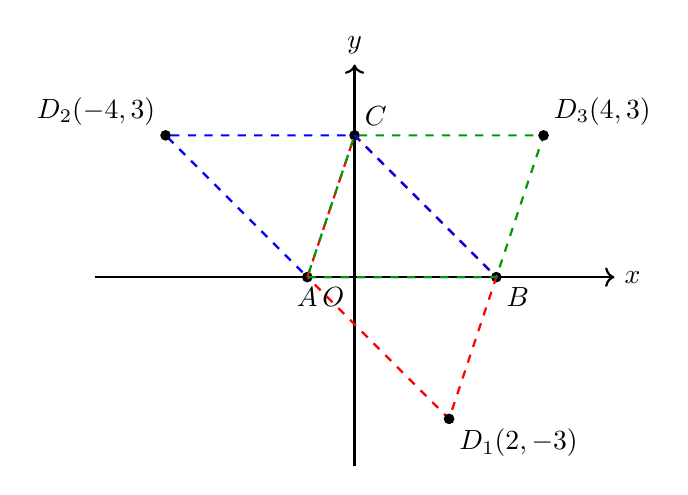
\begin{tikzpicture}[scale=0.6, thick]
  % 坐标轴
  \draw[->] (-5.5, 0) -- (5.5, 0) node[right] {$x$};
  \draw[->] (0, -4) -- (0, 4.5) node[above] {$y$};
  \node[below left] at (0,0) {$O$};

  \coordinate (A) at (-1, 0);
  \coordinate (B) at (3, 0);
  \coordinate (C) at (0, 3);
  \coordinate (D1) at (2, -3);
  \coordinate (D2) at (-4, 3);
  \coordinate (D3) at (4, 3);

  \filldraw (A) circle (2.5pt) node[below] {$A$};
  \filldraw (B) circle (2.5pt) node[below right] {$B$};
  \filldraw (C) circle (2.5pt) node[above right] {$C$};

  % 三个平行四边形
  % ABCD1 (AB, CD1 对角线): 顶点序 A, C, B, D1
  \draw[red, dashed] (A) -- (C) -- (B) -- (D1) -- cycle;
  % AD2CB (AC, BD2 对角线): 顶点序 A, B, C, D2? 对角线 AC, BD2 ⇒ 顶点序 A, B, C, D2
  \draw[blue, dashed] (A) -- (B) -- (C) -- (D2) -- cycle;
  % ABCD3 (AD3, BC 对角线): 顶点序 A, B, D3, C
  \draw[green!60!black, dashed] (A) -- (B) -- (D3) -- (C) -- cycle;

  \filldraw (D1) circle (2.5pt) node[below right] {$D_1(2,-3)$};
  \filldraw (D2) circle (2.5pt) node[above left] {$D_2(-4,3)$};
  \filldraw (D3) circle (2.5pt) node[above right] {$D_3(4,3)$};
\end{tikzpicture}
\end{document}
